\subsection{Der Raetea Forest}

Der Raetea Forest


\begin{figure}[H]
	\centering
	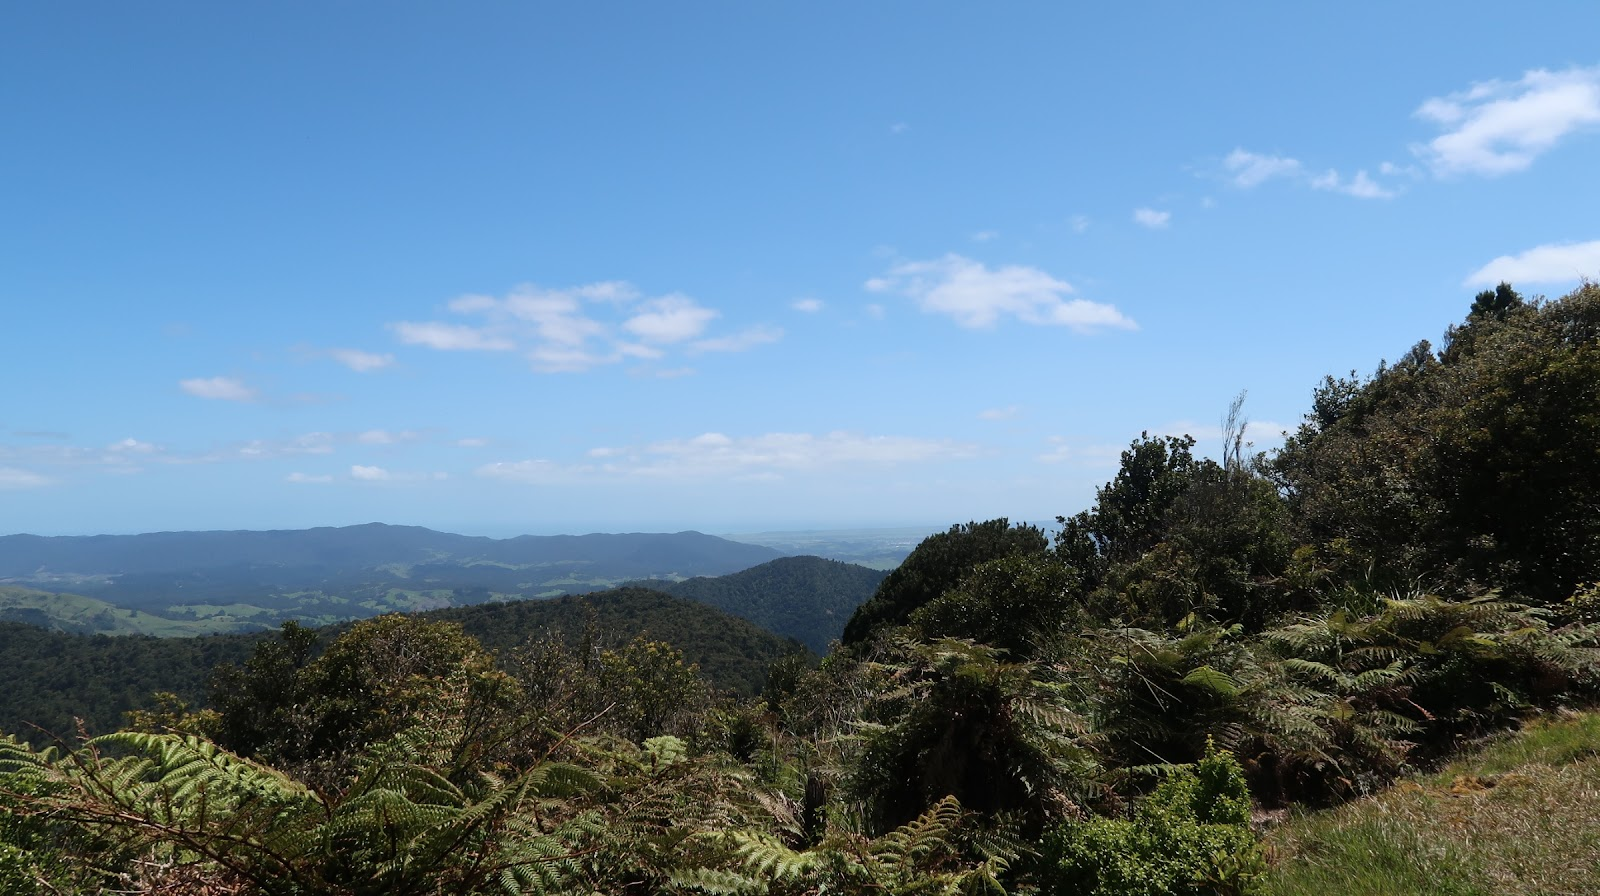
\includegraphics[width=0.5\textwidth]{der_raetea_forest/6_1666810308559623-0.png}
	\caption{}
	\label{fig:6_1666810308559623-0}
\end{figure}

   So 23.10.22    Tag 7
  


   Raetea Forest - Makene Rd
  


  Km  136, 7 - 153, 7
 


\begin{figure}[H]
	\centering
	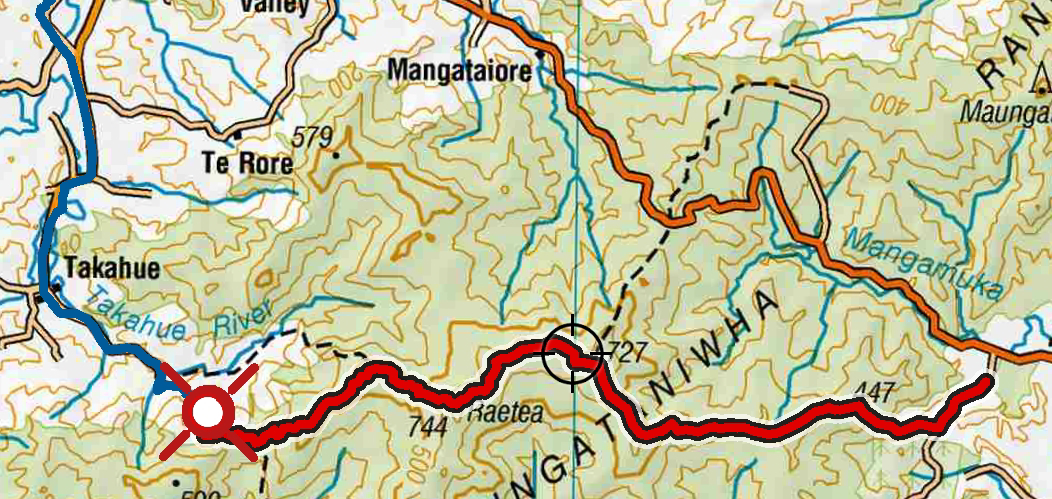
\includegraphics[width=0.5\textwidth]{der_raetea_forest/7_1666810240957561-0.png}
	\caption{}
	\label{fig:7_1666810240957561-0}
\end{figure}

  Jeder der den Te Araroa gewandert ist wird bestimmte Abschnitte nicht mehr vergessen, wie beispielsweise das Tongario Crossing, die Tararua Ranges, die Richmond Ranges und den RAETEA Forest 🥶. Die erst genannten wegen der tollen Aussichten, der gigantischen Landschaften, - der Raetea Forest wegen seiner schlammigen Wege. Wege, die auf etwa 16 km einen Wald/Busch durchstreifen, immer der Kammlinie des Gebirgszuges folgend, Wege die steil bergauf und bergab führen und meist so matschig sind, als würde man auf dem, 'Lieblingssuhlplatz" einer Horde Wildschweine wandern.
 


  Stop...
 


  Noch wissen wir ja gar nicht ob wir wieder in den Genuss dieses neuseeländischen Premiumwanderweges kommen dürfen, es droht ja noch -  "Plan B".
 


  Nach einem Besuch der Bodendeckeltoilette, starten wir relativ spät, gegen 8:00 Uhr hinauf zum Takahue Saddle. Wir füllen noch etwa 1,5 Liter Wasser am letzten Bach auf, im Forest gibt es keine Wasserstelle. Schon bald erreichen wir den Sattel. Mit großen orangenen Dreiecken und einem Hinweisschild ist die Plan B Route gekennzeichnet, nach links führt der Weg in den Wald, auch bei "ungenauem" betrachten der Schilder,  können wir nichts von "gesperrt" lesen.
 


  Also ab nach links...
 


  Wie beschrieben führt der Weg schon bald steil nach oben, zwar schlammig, aber nicht so schlimm wie vor vier Jahren, mittlerweile steht nach jedem Kilometer ein blauer Pfosten mit dem jeweiligen Kilometerstand. Wir brauchen teilweise für einen Kilometer fast eine Stunde.
 


\begin{figure}[H]
	\centering
	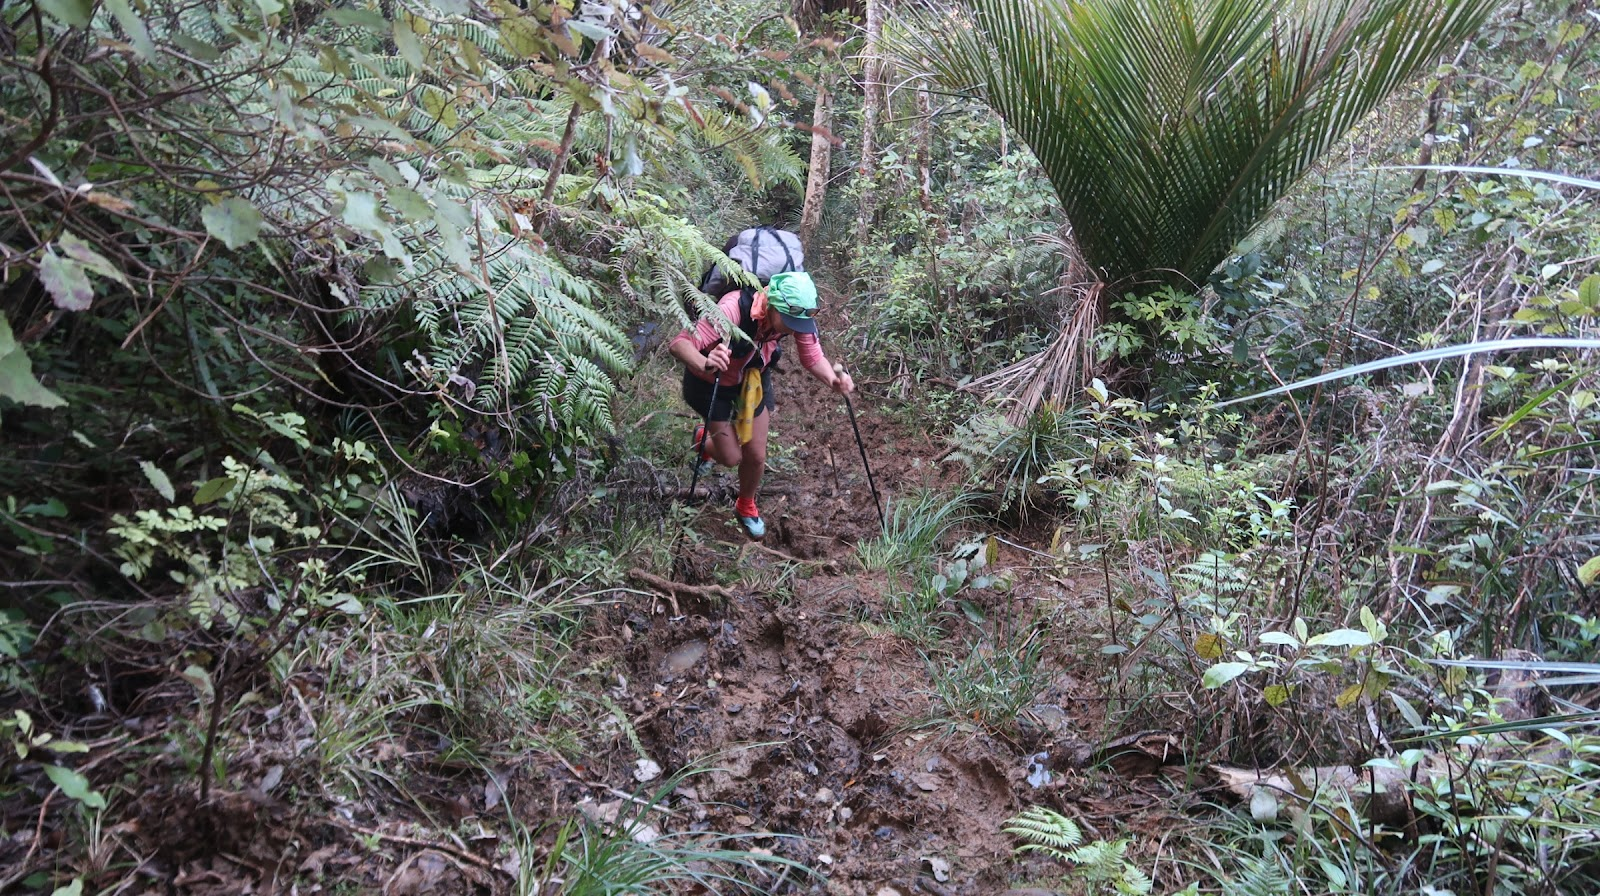
\includegraphics[width=0.5\textwidth]{der_raetea_forest/8_1666810234318588-1.png}
	\caption{}
	\label{fig:8_1666810234318588-1}
\end{figure}

  Nach fast vier Stunden ohne Pause sind wir immer noch nicht auf dem 744 m hohen Summit angekommen. Völlig schlapp, legen wir kurz vor dem Gipfel eine kurze Nuss-Pause ein. Schließlich schaffen wir es doch noch und schleppen uns zu der Radiosendestation, auf dem höchsten Punkt. Nach mehreren Stunden in einem dichten grünen Tunnel, haben wir erstmals wieder einen Ausblick. Wir könnten den Ninety Mile Beach erkennen und einen Blick auf den umliegenden Busch werfen.
 


\begin{figure}[H]
	\centering
	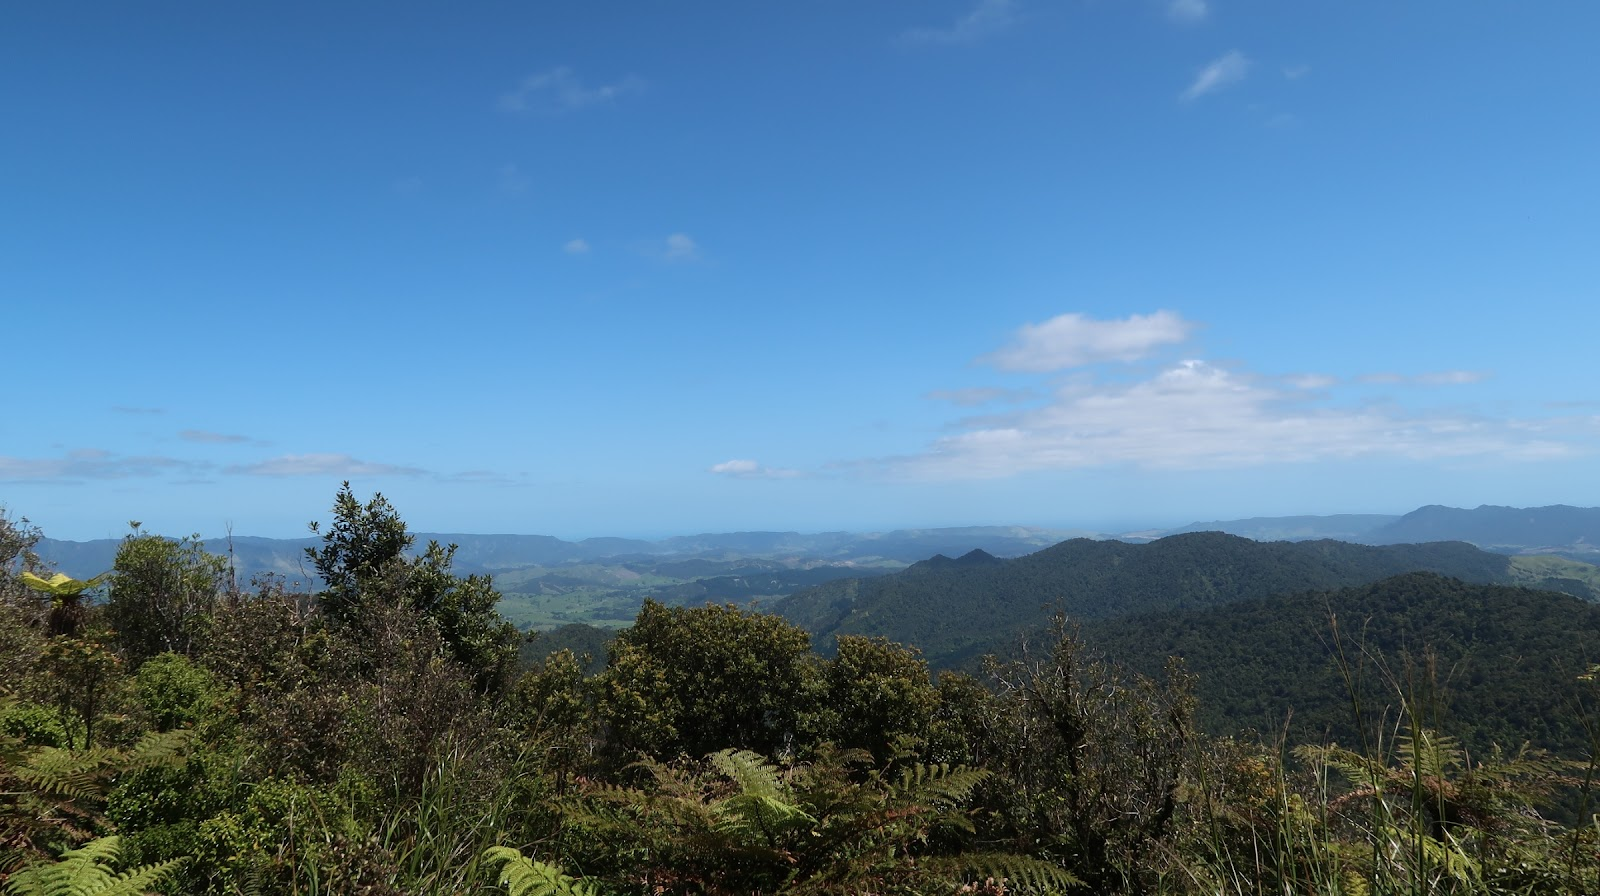
\includegraphics[width=0.5\textwidth]{der_raetea_forest/9_1666810229410207-2.png}
	\caption{}
	\label{fig:9_1666810229410207-2}
\end{figure}

\begin{figure}[H]
	\centering
	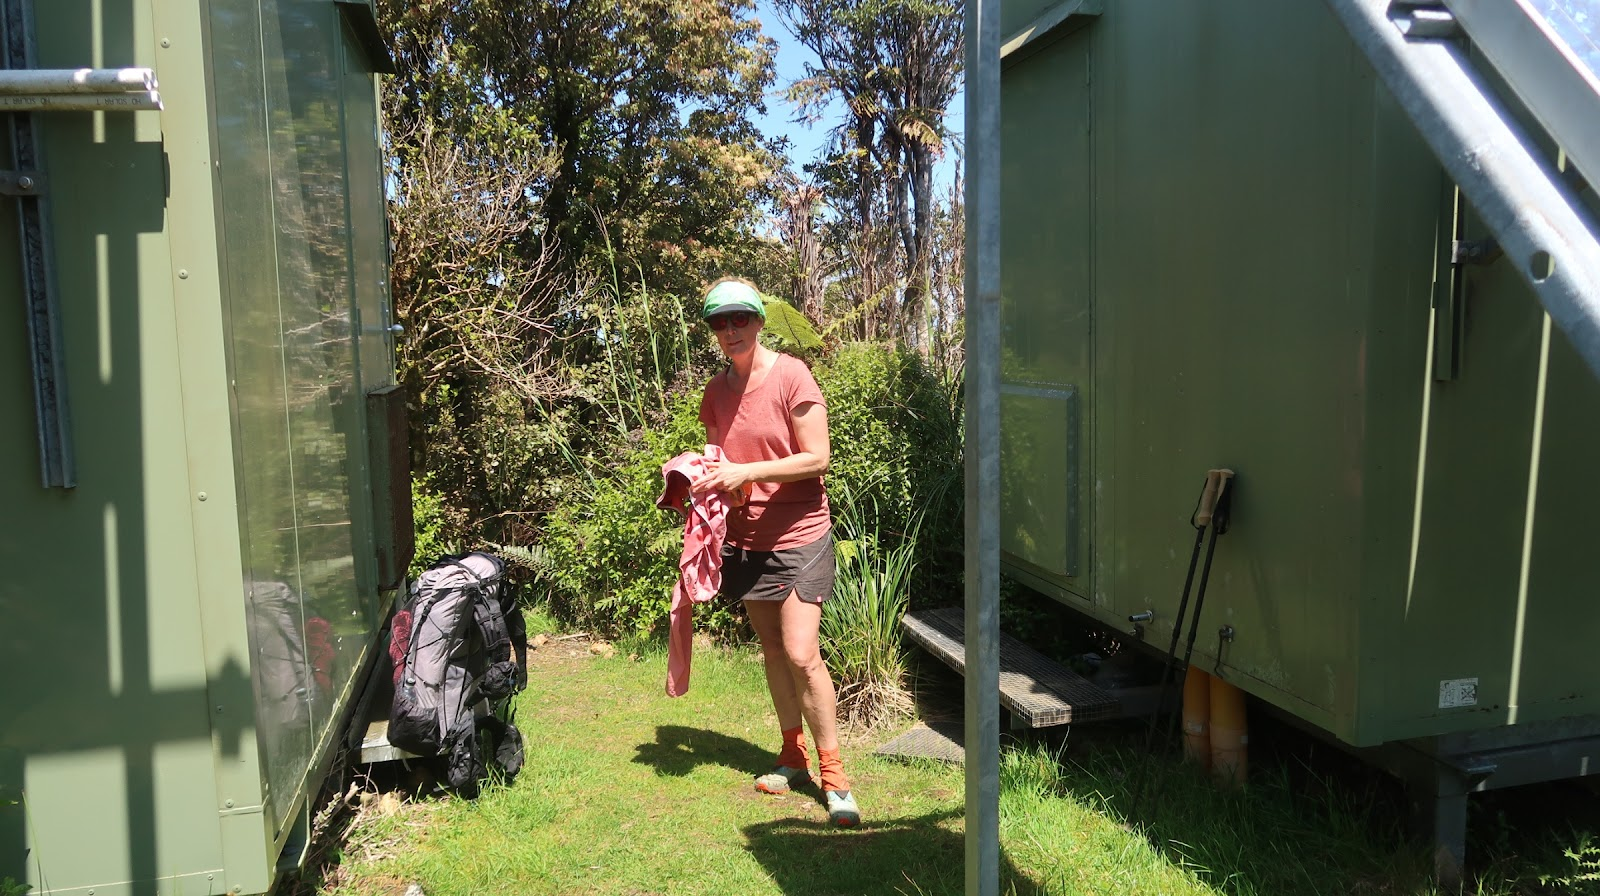
\includegraphics[width=0.5\textwidth]{der_raetea_forest/10_1666810224419060-3.png}
	\caption{}
	\label{fig:10_1666810224419060-3}
\end{figure}

  Im Schatten unter der Solaranlage des Senders machen wir erstmal ein kurzes Mittagsschläfchen. Doch schon bald müssen wir wieder weiter um vor der Dunkelheit den Busch verlassen zu können. Der Weg bergab ist weniger matschig, auch liegen dieses Mal nur wenige Bäume im Weg.
 


  Trotzdem ist es fast 19:00 Uhr als wir endlich den Wald verlassen.
 


  Jetzt müssen wir lediglich die bei TA Hikern berüchtigte Farm, mit den unzähligen, kläffenden Hunden überstehen. Hier hat der Farmer jedoch einen neuen Weg angelegt, um die Hofstelle umlaufen zu können . Jetzt sind es nur noch ein paar hundert Meter und wir erreichen das sichere  Camp direkt am Fluss. Hier treffen wir wieder auf Wang und Remi, einen jungen Franzosen. Die, die Plan B Variante, auch nicht verstehen wollten.
 


  Heute bleibt sogar noch Zeit für ein NFG, danach fallen wir jedoch schon bald in einen tiefen, tiefen Schlaf...
 


\begin{figure}[H]
	\centering
	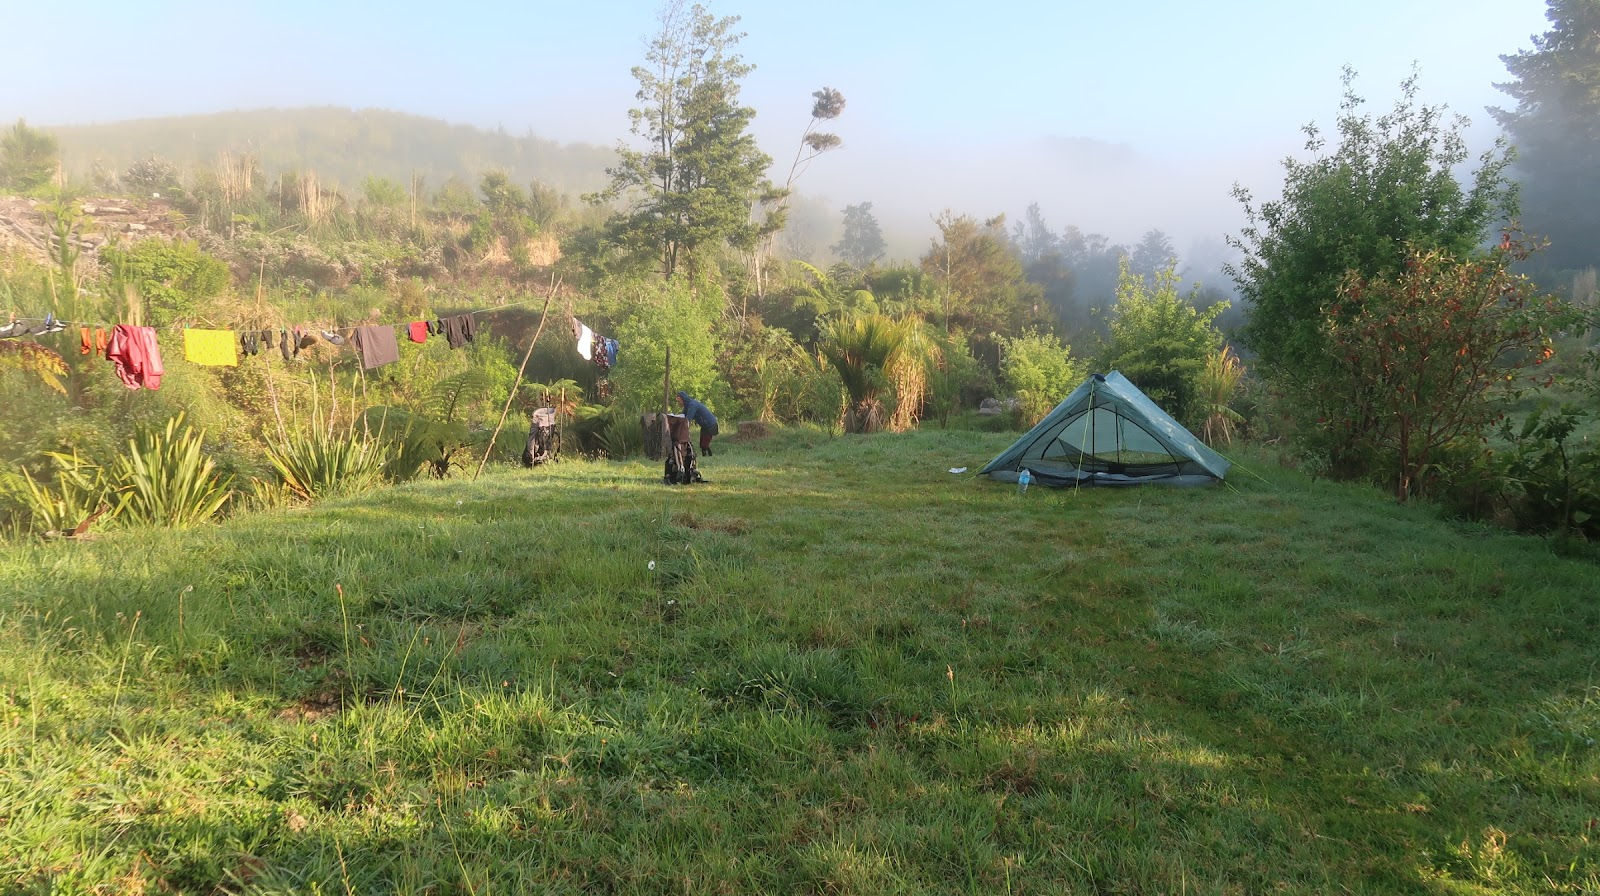
\includegraphics[width=0.5\textwidth]{der_raetea_forest/11_1666810218134476-4.png}
	\caption{}
	\label{fig:11_1666810218134476-4}
\end{figure}

  gelaufene 17 km
 


  in etwa 11 Stunden
 

